%%%%%%%%%%%%%%%%%%%%%%%%%%%%%%%%%%%%%%%%%%%%%%%%%%%%%%%%%%%%%%%%%%%%%%%%%%%%%%%%%%%%%%%%%%%%%%%%%%%%%%%%
\section{ISP Modeling}
\label{sec:modeling}

In this section, a procedure for deriving the kinematic and dynamic models of an ISP installed on a moving base. 

%%%%%%%%%%%%%%%%%%%%%%%%%%%%%%%%%%%%%%%%%%%%%%%%%%%%%%%%%%%%%%%%%%%%%%%%%%%%%%%%%%%%%%%%%%%%%%%%%%%%%%%%
\subsection{Notations and Conventions}
\label{sec:definitions}

This section presents the notations and conventions used in this work. Let $\mathbb{N} = \{0,1,2,\dots\}$ denote the set of \textit{natural numbers} and define $\mathbb{\bar{N}} = \{ \bar{0}\,,\bar{1}\,, \bar{2}\,, \hdots \}$. Unless otherwise stated, $i, j, k \in \mathbb{N} \cup \mathbb{\bar{N}} \cup \{s,c\}$.
%
%\begin{figure}[ht]
    %\centering
    %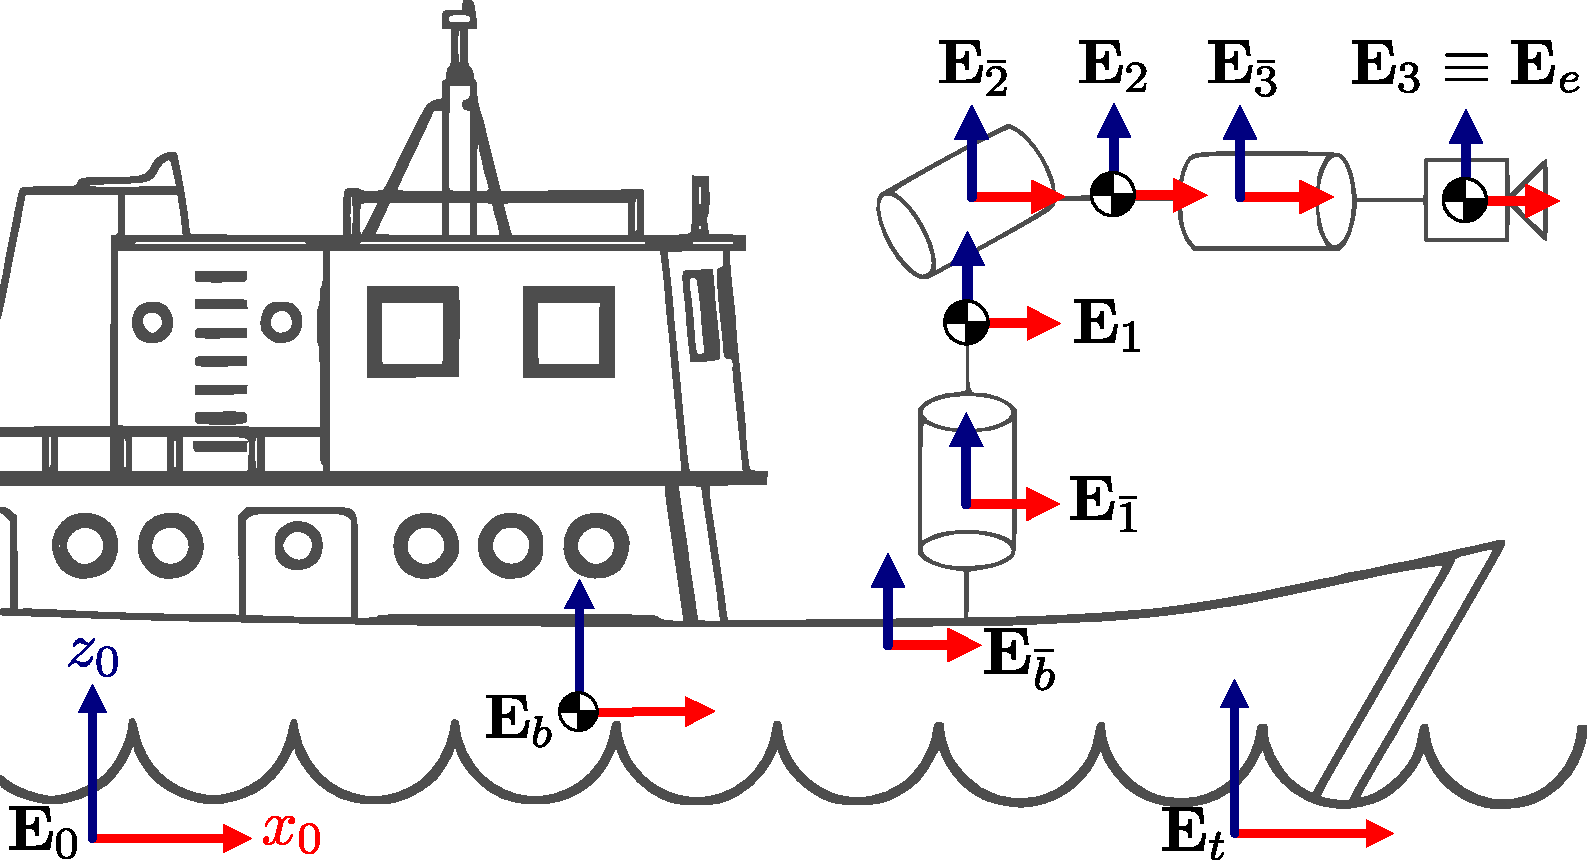
\includegraphics[width=1\columnwidth]{figs/ship_conventions.pdf}
    %\caption{Frame conventions for a 3-DOF ISP system installed on a vessel.}
    %\label{fig:HEADS_convention}
%\end{figure}
%
Define the following:
% coordinate frames, matrices, vectors and scalars:
%
\begin{itemize}
\item $\mathbf{E}_{w}$: world frame, arbitrarily located;
%\item $\mathbf{E}_{s}$: INS frame, placed anywhere on the vehicle or on the last link for the indirect and direct stabilization configurations, respectively;
%\item $\mathbf{E}_{s}$: INS frame, placed anywhere on the system;
\item $\mathbf{E}_{\bar{i}}$: frame fixed on body $i$ with origin on its center of gravity (CG) ($i \in \mathbb{N}_0$);
\item $\mathbf{E}_{i}$: fixed on body $i$ with origin on joint $i$ axis $(i \in \mathbb{N}_0)$;
%\item $\mathbf{E}_{b}$: vehicle frame, placed anywhere on the vehicle. 
%We consider $\mathbf{E}_b \equiv \mathbf{E}_s$ (or $\mathbf{E}_b$ located on $\mathbf{E}_1$) for the indirect (or direct) configuration;
\item $\mathbf{E}_{c}$: camera frame, fixed on the last link;
%\item $\mathbf{E}_{t}$: fixed on the target georeferenced position;
%\item $R_{ij} \in SO(3)$: rotation matrix describing the orientation of frame $\mathbf{E}_j$ relative to frame $\mathbf{E}_i$;
%Of course, $R_{i,i} = I_{3}$, where $I_{3} \in \mathbb{R}^{3 \times 3}$ is the identity matrix;
%
\item $x^k_i\,,y^k_i\,,z^k_i \in \mathbb{R}^{3}$: $\mathbf{E}_i$ canonical unit vectors, written in $\mathbf{E}_k$;
%
%\item $p_{0i} \in \mathbb{R}^{3}$: inertial position of the origin of frame $\mathbf{E}_i$;
%
\item $p^{k}_{ij} \in \mathbb{R}^{3}$: position vector from the origin of frame $\mathbf{E}_i$ to the origin of $\mathbf{E}_{j}$, represented in $\mathbf{E}_k$;
%We use $r=p$ for position and $r=v$ for linear velocity, for example;
%
\item $v^{k}_{ij} \in \mathbb{R}^{3}$: linear velocity from $\mathbf{E}_i$ to  $\mathbf{E}_{j}$, written in $\mathbf{E}_k$;
%
\item $\omega^{k}_{ij} \in \mathbb{R}^{3}$: angular velocity from $\mathbf{E}_i$ to $\mathbf{E}_{j}$, written in $\mathbf{E}_k$;
%
%\item $V^{k}_{ij} = [\, {v^{k}_{ij}}^{T} \,\,\, {\omega^{k}_{ij}}^{T} \,]^T \in \mathbb{R}^{6}$: velocity twist (linear and angular velocities) from $\mathbf{E}_i$ to  $\mathbf{E}_{j}$, written in $\mathbf{E}_k$;
%
%\item $g_{ij} \in SE(3)$: homogeneous transformation matrix from frame $\mathbf{E}_j$ to frame $\mathbf{E}_i$;
%%depending on $R_{ij}$ and on the position vector $p^i_{ij}$;
%
\item $h^{k}_{i} \in \mathbb{R}^{3}$: unit vector defining the rotation axis of joint $i$, represented in $\mathbf{E}_k$ ($i \in \mathbb{N}^*$);
%
%\item $\omega_i \in \mathbb{R}^{3}$: angular velocity of body $i$ seen and represented in the inertial frame 					 $\mathbf{E}_0$ ($i \in \mathbb{N}_1 \cup \{b\}$). Mathematically, $\omega_i$ is defined as the twist coordinates of the $so(3)$ 			 Lie algebra as $\hat{\omega}_i = \dot{R}_i R^{T}_{i}$;

\item $m_i \in \mathbb{R} ,\, I^{i}_{i} \in \mathbb{R}^{3 \times 3}$: mass and inertia tensor of body $i$ represented in $\mathbf{E}_{i}$ ($i \in \mathbb{N}$);
%%
%\item $\overline{I}^i_i =
%\left[\begin{array}{cc}
%\!\! m_i \, I_{3\times3} \!\!&\!\!  0 \!\! \\
%\!\! 0 \!\!&\!\! I^i_i \!\!
%\end{array}\right]$: augmented inertia matrix of body $i$;
%of body $i$ written in $\mathbf{E}_{i} (i \in \mathbb{N}_1 \cup \{b\})$.
%
%\item $\widehat{v}$: $\mathbb{R}^3 \rightarrow so(3)$ cross-product operator;
\item $\mathbf{S}(v) : \mathbb{R}^3 \mapsto \mathrm{so}(3)$ cross product operator;
%
\item $\aket{v}^{\alpha}$: $\mathbb{R}^n \rightarrow \mathbb{R}^n$, where its elements are given by $\aketext{v_i}{\alpha}$, with $v_i \in \mathbb{R}$ ($i = 1,...,n$) being the elements of $v \in \mathbb{R}^n$ and $\alpha \in \mathbb{R}$;
%
\item $\mathbf{I}_{n} \in \mathbb{R}^{n \times n}$: identity matrix of dimension $n$.
%
\end{itemize}
%
%\rev{Also, since the indirect stabilization approach is proposed, the INS frame is supposed to be $\mathbf{E}_{b}$}.
%
%Note that, by the definition of $\mathbf{E}_{i}$, $I^i_i$ is a constant matrix. If $\mathbf{E}_{i}$ is chosen to be aligned with the principal axis of inertia of rigid body $i$, $I^i_i$ is also diagonal.
%Therefore, for simplicity, it is supposed that the principal moments of the inertia matrix of body $i$ are known.
%%
%Also, in the case of a 3-DOF ISP, we suppose that $\mathbf{E}_{e} \equiv \mathbf{E}_{3}$.
%
%%%%%%%%%%%%%%%%%%%%%%%%%%%%%%%%%%%%%%%%%%%%%%%%%%%%%%%%%%%%%%%%%%%%%%%%%%%%%%%%%%%%%%%%%%%%%%%%%%%%%%%%
%\subsection{ISP Modeling}
%\label{sec:modeling}
%
%The \textit{kinematic} model of the ISP can be described by the three equations below:
%%
%\begin{align}
%R_{oc}(\eta_{c_2}) &= R_{ob}(\eta_{b_2}) \, R_{bc}(q) \,, \nonumber \\
%\omega^{c}_{0c} &= J^{B}_{bc}(q) \, \dot{q} + R^{\mathsf{T}}_{bc}(q)\,\omega^{b}_{0b} \,, \nonumber \\
%\dot{\omega}^{c}_{0c} &= J^{B}_{bc}(q) \, \ddot{q} + \dot{J}^{B}_{bc}(q) \, \dot{q} + \dot{\omega}^{c}_{0b} \,.
%\label{eq:outer_model}
%\end{align}
%
%In this section, we summarize the mathematical framework for VMS proposed in \cite{Gravdahl2014}, applying it to find   the
%dynamic model of a 3 DOF ISP.
%
%We consider only the case of manipulators with rotational joints, which is usual in ISPs.
%
%The section is organized as follows. First, we discuss the kinematics of VM systems. Second, the dynamic equations of motion    for a
%general multibody system are presented. Lastly, the dynamic equations of a VM in $SE(3)$ are derived using the 	 previous formulation
%and applied to the case of a 3 DOF ISP.
%
%The section is organized as follows: first, the kinematics of a vehicle-manipulator system is discussed. 		  Second, the ISP dynamic
%equations of motion are derived using the framework of \cite{Gravdahl2014}. Finally, the system equations of motion are derived    by
%means of the Newton-Euler formalism.
%
%In this work, if the superscript symbol is omitted, the vector is represented in the inertial frame, $\mathbf{E}_0$.
%
Let body $0$ be the moving base and bodies $1,2,3$ be the ISP gimbals.
%
Also, if a superscript is omitted, the vector is written in world frame $\mathbf{E}_w$ coordinates.

%%%%%%%%%%%%%%%%%%%%%%%%%%%%%%%%%%%%%%%%%%%%%%%%%%%%%%%%%%%%%%%%%%%%%%%%%%%%%%%%%%%%%%%%%%%%%%%%%%%%%%%%
\subsection{Quaternion-Based Kinematics}

Let $R \in SO(3)$ be a \textit{rotation matrix} describing the rotation from an arbitrary frame to another.
%
Then, $R$ is a diffeomorphism with respect to the projective space $\mathbb{RP}^{3} \!=\! \left\{ \norm{v}^2 \leq \pi \,\,|\,\, v \in \mathbb{R}^3 \right\}$.
%the manifold composed of all points inside a rigid ball of radius $\pi$ centered on the origin of $\mathbb{R}^{3}$. 
Therefore, each point $v \in \mathbb{RP}^{3}$ represent a $4$-parameter representation for $SO(3)$ called the \textit{angle-axis}, where the unitary vector on the direction of $v$ represents the rotation axis and $\norm{v}$ represents the corresponding rotation angle around that axis.
%
\begin{remark}
Note that $\mathbb{RP}^{3}$ covers $SO(3)$ twice, since any point on it actually represents the same rotation than the opposite point of the sphere.
\end{remark}
%
This representation can be expressed by $v = \{\theta,n\}$, where $\theta \in \mathbb{R}$ is the angle of rotation around the unit axis vector $n \in \mathbb{R}^{3}, \norm{n} = 1$.
%
Another non-minimal representation is the \textit{unit quaternion}. The set of \textit{quaternions} $\mathbb{H}$ is defined by:
%
\begin{align}
\mathbb{H} &:= \left\{ \eta + i \epsilon_{1} + j \epsilon_{2} + k \epsilon_{3} \,\,|\,\, \eta,\epsilon_{1},\epsilon_{2},\epsilon_{3} \in \mathbb{R} \right\} \,, \nonumber \\
i^2 &= j^2 = k^2 = ijk = -1 \,.
\label{eq:def_quaternion}
\end{align}

A quaternion $Q \in \mathbb{H}$ can also be represented as the pair $Q := \{\eta,\epsilon\}$, where 
$\eta = \mathsf{Re}(Q) \in \mathbb{R}$ represents the \textit{real} part of the quaternion and $\epsilon = \mathsf{Im}(Q) = [\,\, \epsilon_{1} \,\,\, \epsilon_{2} \,\,\, \epsilon_{3} \,\,]^\mathsf{T} \in \mathbb{R}^{3}$ represents the vector part.
%
The quaternion \textit{conjugate} is given by $Q^* = \{\eta,-\epsilon\}$.
%
One can also represent the quaternion in fully vector form by the notation 
$\bar{Q} = [\,\, \eta \,\,\, \epsilon_{1} \,\,\, \epsilon_{2} \,\,\, \epsilon_{3} \,\,]^\mathsf{T} \in \mathbb{R}^4$.

Quaternions also form an algebraic {\it group} with respect to {\it multiplication}.
Given two quaternions $Q_1=\{\eta_1,\epsilon_1\}$ and $Q_2=\{\eta_2,\epsilon_2\}$, their multiplication follow the rules established by definition \eqref{eq:def_quaternion}, which results in:
%
\begin{align}
Q_1\cdot Q_2 = \{\eta_1\eta_2 - \epsilon_1^\mathsf{T}\epsilon_2 ,\, \eta_1\epsilon_2 + \eta_2\epsilon_1 + \epsilon_1 \times \epsilon_2 \} \,.
\label{eq:quaternion_product}
\end{align}
%
Quaternion multiplication can also be performed as a linear transformation in $\mathbb{R}^4$, by:
%
\begin{align}
\overline{Q_1 \cdot Q_2} &= \mathbf{H}_+(Q_1) \, \overline{Q_2} \,, \\
&= \mathbf{H}_-(Q_2) \, \overline{Q_1} \,,
\label{eq:multipl_Hamilton}
\end{align}
%
where $\mathbf{H}_+$, $\mathbf{H}_-$ are {\it Hamilton operators} defined by:
%
\begin{align}
\mathbf{H}_+(Q) &= \left[ \begin{array}{cc}
\overline{Q} & \mathbf{h}_+(Q)
%\epsilon & \eta \, \mathbf{I}_3 + \widehat{\epsilon}
\end{array} \right], \quad
%
\mathbf{h}_+(Q) = 
\left[ \begin{array}{cc}
-\epsilon^\mathsf{T} \\
\eta \, \mathbf{I}_3 + \widehat{\epsilon}
\end{array} \right] \\
%
\mathbf{H}_-(Q) &= \left[ \begin{array}{cc}
\overline{Q} & \mathbf{h}_-(Q)
\end{array} \right], \quad
%
\mathbf{h}_-(Q) = 
\left[ \begin{array}{cc}
-\epsilon^\mathsf{T} \\
\eta \, \mathbf{I}_3 - \widehat{\epsilon}
\end{array} \right]
\label{eq:Hamilton_op}
\end{align}

The square of the quaternion \textit{norm} is defined as the \textit{scalar}:
%
\begin{align}
\norm{Q}^2 = Q \cdot Q^* = \{ \eta^2 + \epsilon^\mathsf{T} \epsilon , 0 \} \,,
\end{align}
%
and its \textit{inverse} is the quaternion $Q^{-1}$ such that $Q \,\circ\, Q^{-1} = \{1,0\}$, the {\it unitary} quaternion.

The set of \textit{unit quaternions} $\mathbb{H}^* = \{ Q \in \mathbb{R}: \norm{Q} = 1 \}$ can be used as a parametrization for orientation in the following way.
%
For an element $p = \{\theta,n\}\in \mathbb{RP}$, define:
%
\begin{align}
Q = \left\{cos\left(\frac{\theta}{2}\right) \,, sin\left(\frac{\theta}{2}\right)\,n\right\} \in \mathbb{H}^* \,.
\label{eq:quaternion_rotation}
\end{align}
%
The inverse of an unit quaternion is given by $Q^{-1} \!\!=\!\! Q^*$, 
which according to \eqref{eq:quaternion_rotation}, clearly corresponds to the opposite rotation due to negative direction of the rotation axis $n$.

Let $r_0, r_1, ... , r_n \in \mathbb{H}^*$ be the $n$ absolute rotations between frames $\mathbf{E}_0, \mathbf{E}_1, ..., \mathbf{E}_n$ and the world frame $\mathbf{E}_w$, and $r^i_{i+1} \in \mathbb{H}^*$ ($i=1,2,...,n-1$) represent the rotations from frame $\mathbf{E}_i$ to $\mathbf{E}_{i+1}$.
%Note that $r^j_i = (r^i_j)^*$ represents the opposite rotation.
Then, since the unit quaternions form a group with respect to multiplication, then:
%
\begin{align}
r_n = r_1 \cdot r^1_2 \cdot ... \cdot r^{n-1}_n \in \mathbb{H}^* \,.
\end{align}

Now, define the set of \textit{pure} quaternions $\mathbb{H}_p = \{ v \in \mathbb{H}: \mathsf{Re}(v) = 0 \}$.
%
Note that any vector from $\mathbb{R}_3$ can be represented as the vector part of a corresponding element $v \in \mathbb{H}_p$.
%
Besides, note that the following holds for $v,w \in \mathbb{H}_p$:
\begin{align}
%\overline{v \circ w} = \left[ \begin{array}{c}
%-\mathsf{Im}(v)^\mathbf{T} \mathsf{Im}(w) \\ 
%\mathsf{Im}(v) \times \mathsf{Im}(w)
%\end{array} \right] \,.
%
v \cdot w = \{ -\mathsf{Im}(v)^\mathsf{T} \mathsf{Im}(w) ,\,\, \mathsf{Im}(v) \times \mathsf{Im}(w) \} \,.
%
%v \circ w = \{ -v^\mathbf{T} w ,\,\, v \times w \} \,.
\end{align}
%
%were here we interchange the quaternion and vector notation, since each one has a clear meaning in this case.

Let $v^i$ and $v^j \!\in\! \mathbb{H}_p$ be representations for a vector $\vec{v}$ in frames $\mathbf{E}_i$ and $\mathbf{E}_j$, respectively, and $r^i_j$ represents the rotation from $\mathbf{E}_i$ to $\mathbf{E}_j$, with unitary axis $n^i_{j} \in \mathbb{R}^3$ and rotation angle $\theta_{ij}$.
%
Then, the following relation is valid:
%
\begin{align}
v^i = (r^i_j) \cdot v^j \cdot (r^i_j)^* = Ad_{r^i_j} \left[ v^j \right] \,,
\end{align}
%
where $Ad_{r^i_j}[*]$ is the adjoint {\it operator}.
%
Note that, in vector algebra, $Ad_{r^i_j}$ represents the corresponding rotation matrix $R_{ij} \in SO(3)$ associated to the unit quaternion $r^i_j \in \mathbb{H}^*$.
%
In terms of the components of $r^i_j$, this matrix is given by:
%
\begin{align}
R_{ij} = n^i_{j} (n^i_{j})^\mathsf{T} + s_{ij} \, \mathbf{S}(n^i_{j}) + c_{ij} \, (\mathbf{I}_3 - n^i_{j} (n^i_{j})^\mathsf{T}) \,,
\label{eq:quaternion_rotation_matrix}
\end{align}
%
where $s_{ij}$ and $c_{ij}$ are the sine and cosine functions of $\theta_{ij}$.
The rotation matrix corresponding to an absolute rotation $r_i \in \mathbb{H}^*$ is written with only one subscript, as $R_i \in SO(3)$.

%%%%%%%%%%%%%%%%%%%%%%%%%%%%%%%%%%%%%%%%%%%%%%%%%%%%%%%%%%%%%%%%%%%%%%%%%%%%%%%%%%%%%%%%%%%%%%%%%%%%%%%%
\begin{algorithm}[Kinematic Propagation]
The algorithm is initialized with the vessel configuration $p_{00} \in \mathbb{R}^3$ and $r_0 \in \mathbb{H}^*$. 
Then, varying index $i$ from $0$ to $n-1$, the configuration of each frame with respect to the vessel frame $\mathbf{E}_0$ can be computed by:
%
%\begin{align}
%p_{0,i+1} &= p_{0,i} + Ad_{r_i} \left[\, p^i_{i,i+1} \,\right] \,, \\
%r_{i+1} &= r_i \circ r^i_{i+1} \,.
%\end{align}
%%
%or still, using vector notation:
%
\begin{align}
p_{0,i+1} &= p_{0,i} + R_{i} \, p^i_{i,i+1} \,, \\
\overline{r}_{i+1} &= \mathbf{H}_+(r_i) \, \overline{r}^i_{i+1} \,.
\end{align}
%
with $R_i$ computed from $r_i$ in \eqref{eq:quaternion_rotation_matrix}.
The camera pose can be computed as $p_{0c} = p_{0n} + R_{c} \, p^n_{nc}$, $r_c = \mathbf{H}_+(r_n) \, \overline{r}^n_{c}$.
%
\end{algorithm}

%The homogeneous transformation matrix $g_{wi}(p_{wi},R_{wi}) \in SE(3)$ associated to $\mathbf{E}_{i}$ relative to $\mathbf{E}_{w}$ is:
%%
%\begin{equation}
%g_{wi}(p_{wi},R_{wi}) = \left[\begin{array}{cc}
%R_{wi} & p_{wi} \\
  %0    &   1
%\end{array}\right] \,.
%\label{eq:g_0b}
%\end{equation}
%%where $R_{0b}$ is the vehicle rotation matrix.
%%
%If $\mathbf{E}_{i}$ is a frame fixed on a link, its pose is given by the group operation among $SE(3)$ elements:
%%
%\begin{align}
%g_{0i} = g_{0b}(p_{0b},R_{0b}) \, g_{bi}(q) \,,
%\end{align}
%%
%where $q$ is the vector of joint positions and $g_{bi}(q)$ is the \textit{forward kinematics map} from the vehicle frame $\mathbf{E}_{b}$ to $\mathbf{E}_{i}$.

Let $\vec{v}_{i}$ and $\vec{\omega}_{i}$ be the physical linear and angular velocities of $\mathbf{E}_{i}$. They are represented by 
%$v_{0i} = \dot{p}_{0i}\in\mathbb{R}^{3}$ and $\omega_{0i}\in\mathbb{R}^{3}$ when written in inertial coordinates and by $v^{i}_{0i}\in\mathbb{R}^{3}$ and 
$v^{i}_{i}\in\mathbb{R}^{3}$ and $\omega^{i}_{i}\in\mathbb{R}^{3}$ when written in its own body frame.
%
Let $r_i = \{\eta_i,\epsilon_i\}\in\mathbb{H}^*$ be the absolute rotation of $\mathbf{E}_i$. 
%In the same way that $\widehat{\omega}^i_{0i} = R^\mathsf{T}_{0i}\,\dot{R}_{0i}\in so(3)$ is the \textit{Lie algebra} of $SO(3)$
The time-derivative of $r_i$ can be related to $\omega^i_{i}$ by:
%
\begin{align}
\dot{\overline{r}}_i = 
%
\left[ \begin{array}{cc}
\dot{\eta}_i \\
\dot{\epsilon}_i 
\end{array} \right] = 
%
\frac{1}{2} \, \left[ \begin{array}{cc}
- \epsilon_i^\mathsf{T} \\
\eta_i\,\mathbf{I}_3 + \widehat{\epsilon}_i
\end{array} \right] \, \omega^i_{i} \,, 
\label{eq:quaternion_propagation}
\end{align}
%
which is known as the \textit{quaternion propagation} formula.

The vector $V^{i}_{i} = [\, (v^{i}_{i})^\mathsf{T} \,\,\, (\omega^{i}_{i})^\mathsf{T} \,]^\mathsf{T} \in \mathbb{R}^{6}$ is the \textit{body velocity twist} associated to $\mathbf{E}_{i}$.
%
Two body velocity twists associated to different frames $\mathbf{E}_i$, $\mathbf{E}_j$ located in the \textit{same rigid-body} are related through the constant adjoint map 
$Ad_{g_{ij}} \in \mathbb{R}^{6 \times 6}$:
%
\begin{equation}
V^{i}_{i} = Ad_{g_{ij}} V^{j}_{j} \,, \quad
%
Ad_{g_{ij}} =
\left[\begin{array}{cc}
R_{ij} & \hat{p}^{i}_{ij} \, R_{ij} \\
  0    &             R_{ij}
\end{array}\right] \,.
\label{eq:adjoint_map}
\end{equation}
%
which has the property $Ad_{g_{ji}} = Ad^{-1}_{g_{ij}}$.

%such that its Lie algebra is given by $\widehat{V}^{i}_{0i} = g_{0i}^{-1} \, \dot{g}_{0i} \in se(3)$.
%%
%One can also define the \textit{spatial velocity twist} $V^{S}_{0i} \in \mathbb{R}^{6}$, such that $\widehat{V}^{S}_{0i} = \dot{g}_{0i} \, g_{0i}^{-1} \in se(3)$. However, recall that $V^{S}_{0i}$ is not the same as $V_{0i}$, which is the velocity of $\mathbf{E}_i$ written in $\mathbf{E}_0$.
%%
%Two general spatial and body velocity twists are related through the adjoint map $Ad_{ij}(g_{ij}) \in \mathbb{R}^{6 \times 6}$:
%%
%\begin{equation}
%V^{S}_{ij} = Ad_{ij} V^{j}_{ij} \,, \quad
%%
%Ad_{ij} =
%\left[\begin{array}{cc}
%R_{ij} & \hat{p}^{i}_{ij} \, R_{ij} \\
  %0    &             R_{ij}
%\end{array}\right] \,,
%\label{eq:adjoint_map}
%\end{equation}
%%
%which has the property $Ad_{ji} = Ad^{-1}_{ij}$.
%
Now, given the body twists $V^0_{0}$ and $\dot{V}^0_{0}$ of frame $\mathbf{E}_0$ in the ship, it is possible to compute all velocities $V^i_{i}$ and accelerations $\dot{V}^i_{i}$ associated to each link ($i=1,2,3$) by means of an iterative algorithm described below. It consists in propagating the body velocity/acceleration twists of each link frame $\mathbf{E}_{i}$ through the system, obtaining $V^{i}_{i}$, $\dot{V}^{i}_{i}$, $i \in \{1,2,3\}$.

%%%%%%%%%%%%%%%%%%%%%%%%%%%%%%%%%%%%%%%%%%%%%%%%%%%%%%%%%%%%%%%%%%%%%%%%%%%%%%%%%%%%%%%%%%%%%%%%%%%%%%%
\begin{algorithm}[Propagation of Velocities and Accelerations]
\label{alg:forward_propagation}

The algorithm is initialized with given $V^{0}_{0}$, $\dot{V}^{0}_{0}$.
%
%The algorithm is initialized with $V^{0}_{00} = V^{b}_{0b}$, $\dot{V}^{0}_{00} = \dot{V}^{b}_{0b} - g\,[\, z^\mathsf{T}_0 R_{0b} \,\,\,\, 0^\mathsf{T} \,]$, accounting the effects of gravity.
%
%If the INS is placed on the vehicle, we compute the propagating \textit{upwards}, from the vehicle to the last link, according to:
%
%If the INS is placed in the vehicle ($n$-th link), the propagation starts in the vehicle ($n$-th link) to the last link (vehicle).
%
%The propagation algorithm can be split into two: the \textit{upward} and \textit{downward} parts. The \textit{upward} propagation equations are given by:
%
%If the INS is located on the vehicle (indirect stabilization, $k=b$), the algorithm is initialized with $V^{0}_{00} = V^{s}_{0s}$, $\dot{V}^{0}_{00} = \dot{V}^{s}_{0s}$, and the propagation goes \textit{upwards} the kinematic chain through the following equations:
%
%The algorithm is initialized with the motion variables of frame $\mathbf{E}_b$. 
%
Then, the velocities and accelerations are propagated \textit{upwards} the kinematic chain from $i=0$ until $i=n=3$:
%
\begin{flalign}
V^{i}_{i} &= \Omega_{i-1,i}^\mathsf{T} \, ( \Phi_{i,i-1} \, V^{i-1}_{i-1} + H_{i} \, \dot{q}_{i} ) \,, \label{eq:upwards_prop1} \\
%
\dot{V}^{i}_{i} &= \Omega_{i-1,i}^\mathsf{T} \, ( \Phi_{i,i-1} \, \dot{V}^{i-1}_{i-1} + H_{i} \, \ddot{q}_{i} + A_{i} \, \dot{q}_{i} ) \,.
\label{eq:upwards_prop2}
\end{flalign}
%
%The algorithm is initialized with $V^{0}_{00} = V^{s}_{0s}$, $\dot{V}^{0}_{00} = \dot{V}^{s}_{0s}$ and starts from $i-1$ being the link where the INS is placed until $i = n$.
%
The velocity/acceleration twists of the camera are computed by $V^c_{c} = Ad_{g_{cn}} \, V^{n}_{n}$, $\dot{V}^c_{c} = Ad_{g_{cn}} \, \dot{V}^{n}_{n}$, with a constant transformation $g_{cn}$.
%
%Then, the velocities and accelerations are propagated \textit{downwards} from frame $\mathbf{E}_{i+1}$, where $\mathbf{E}_k$ is attached to, until $i=0$. The equations are given by inverting \eqref{eq:upwards_prop1} and \eqref{eq:upwards_prop2}:
%
%where $i = 1, \ldots, n$. %The camera velocity/acceleration twists are computed by $V^c_{0c} = Ad_{g_{cn}} \, V^{n}_{0n}$, $\dot{V}^c_{0c} = Ad_{g_{cn}} \, \dot{V}^{n}_{0n}$.
%
%The \textit{downward} propagation equations are given by simply inverting \eqref{eq:upwards_prop1} and \eqref{eq:upwards_prop2}:
%If the INS is on the last link (direct stabilization, $k=c$), the algorithm is initialized with $V^{n}_{0n} = Ad_{g_{ns}} \, V^{s}_{0s}$, $\dot{V}^{n}_{0n} = Ad_{g_{ns}} \, \dot{V}^{s}_{0s}$, with $i = n-1, \ldots, 1$.
%
%In this case, the velocity/acceleration twists are propagated \textit{downwards} through equations given by simply inverting \eqref{eq:upwards_prop1} and \eqref{eq:upwards_prop2}:
%
%\begin{flalign}
%V^{i}_{0i} &= \Phi^{-1}_{i+1,i} \, ( \Omega_{i,i+1} \, V^{i+1}_{0,i+1} - H_{i+1} \, \dot{q}_{i+1} ) \label{eq:downwards_prop1} \\
%%
%\dot{V}^{i}_{0i} &= \Phi^{-1}_{i+1,i} \, ( \Omega_{i,i+1} \, \dot{V}^{i+1}_{0,i+1} - H_{i+1} \, \ddot{q}_{i+1} - A_{i+1} \, \dot{q}_{i+1} ) \,.
%\label{eq:downwards_prop2}
%\end{flalign}
%
The matrices in \eqref{eq:upwards_prop1}, \eqref{eq:upwards_prop2} are given by:
%
\begin{alignat*}{3}
&\Phi_{i+1,i} &=& \mat{
\mathbf{I}_{3} \!\!&\!\! -\mathbf{S}(p^{i}_{i,i+1}) \\
0     \!\!&\!\! \mathbf{I}_{3}
}, \quad \quad
%
\Phi^{-1}_{i+1,i} &=& \mat{
\,\, \mathbf{I}_{3} \!\!&\!\! \mathbf{S}(p^{i}_{i,i+1}) \\
0     \!\!&\!\! \mathbf{I}_{3}
}, \\
%
&H^\mathsf{T}_{i+1} &=& \mat{ 
0^\mathsf{T} \!\!\!&\!\!\! ( h^{i}_{i+1} )^\mathsf{T}
} \quad \,\,\,\,, \quad \quad
%
%R_{i\,,i+1} &=& \exp(\mathbf{S}(h^{i}_{i+1}) \, q_{i+1})\,, \\
%
\Omega_{i,i+1} &=& \mat{ 
R_{i,i+1} \!\!\!&\!\!\! 0         \\ 
0          \!\!\!&\!\!\! R_{i,i+1} 
}\,\,\,\,,\\
%
&A_{i+1} &=& \mat{
\mathbf{S}(v^{i}_{0i} + \mathbf{S}(\omega^{i}_{0i}) \, p^{i}_{i,i+1}) \, h^{i}_{i+1} \\
\mathbf{S}(\omega^{i}_{0i}) \, h^{i}_{i+1} }
\end{alignat*}
%
%\begin{alignat*}{3}
%&\Phi_{i+1,i} &&= \mat{
%\,\, \mathbf{I}_{3} \!\!&\!\! -\hat{p}^{i}_{i,i+1} \\
%0     \!\!&\!\! \mathbf{I}_{3}
%},
%%
%\quad \,\,\,\, \Phi^{-1}_{i+1,i} &&= \mat{
%\,\, \mathbf{I}_{3} \!\!&\!\! \hat{p}^{i}_{i,i+1} \\
%0     \!\!&\!\! \mathbf{I}_{3}
%}, \\
%%
%& H^\mathbf{T}_{i+1} &&= \mat{ 
%0^\mathbf{T} \!\!\!&\!\!\! ( h^{i}_{i+1} )^\mathbf{T}
%} ,
%%
%\quad \quad \Omega_{i,i+1} &&= \mat{ 
%R_{i,i+1} \!\!\!&\!\!\! 0         \\ 
%0          \!\!\!&\!\!\! R_{i,i+1} 
%}, \\
%%
%&A_{i+1} &&= \mat{
%(\hat{v}^{i}_{0i} + \reallywidehat{\hat{\omega}^{i}_{0i} \, p^{i}_{i,i+1}}) \, h^{i}_{i+1} \\
%\hat{\omega}^{i}_{0i} \, h^{i}_{i+1} } \,,
%\end{alignat*}
%
where the rotation matrices $R_{i,i+1}$ are computed from 
$r_{i,i+1} = \left\{ cos\left(\frac{1}{2} q_{i+1}\right), h^i_{i+1}\,sin\left(\frac{1}{2} q_{i+1}\right) \right\} \in \mathbb{H}^*$
using \eqref{eq:quaternion_rotation_matrix}.

\end{algorithm}

%Note that this algorithm can be generalized to be initialized with twists anywhere on the system, and not just on the first or last body, given that the two procedures are followed.

%Therefore, the relation between the ship spatial and body twists $V^{S}_{0b}$ and $V^{b}_{0b}$ is given by $V^{S}_{0b} = Ad_{g_{0b}} V^{b}_{0b}$, where $Ad_{g_{0b}}$ is the adjoint map corresponding to $g_{0b}(\eta)$.
%
%Further details can be found in \cite{Murray1994}.

Now, recall that $\omega^{i}_{i}$ can be written as the sum $\omega^{i}_{i} = \omega^{i}_{0} + \omega^{i}_{0,i}$
%where $\omega^{i}_{bi}$ is the body velocity associated to $\mathbf{E}_i$ relative to the vehicle frame $\mathbf{E}_b$.
%
and can be expressed in terms of $q\,,\dot{q}\in\mathbb{R}^{3}$ by means of the \textit{angular body link Jacobian} $J^i_{0i}(q,\Pi_g) \in \mathbb{R}^{3 \times 3}$ as $\omega^{i}_{0,i} = J^{i}_{0i}(q,\Pi_g) \, \dot{q}$:
%and of $R_{0i}(q)$ as $\omega^i_{0} = R^\mathsf{T}_{0i}(q,\Pi_g) \, \omega^{0}_{0}$:
%
%This velocity vector can be expressed in terms of $\dot{q}$ by means of the body link Jacobian $J^i_i(q) \in \mathbb{R}^{6 \times n}$:
%%
%\begin{equation}
%V^{i}_{bi} = J^{i}_i(q) \, \dot{q} \,,
%\label{eq:geometric_Jacobian}
%\end{equation}
%%
%yielding
%
\begin{align}
\omega^{i}_{i} &= J^{i}_{0i}(q,\Pi_g) \, \dot{q} + \omega^{i}_{0} \,,
\label{eq:gen_vel_transform1}
\end{align}
%
where $\Pi_g$ is the vector of {\it geometric} parameters of the ISP, containing combinations of components of the axes and distance vectors of each link frame.
%
Note that the body link Jacobian $J^i_{0i}(q,\Pi_g)$ can be computed numerically from \eqref{eq:upwards_prop1},
%
%\begin{align}
%J^i_{bi}(q) = \mat{
%R^\mathsf{T}_{bi} \, h^b_1 \!\!&\!\!\! R^\mathsf{T}_{1i} \, h^1_2 \!\!&\!\!\! \cdots \!\!\!&\!\! R^\mathsf{T}_{ii} \, h^i_{i+1} \!\!&\!\! 0_{3 \times (3-i)} },
%\label{eq:link_body_jacobian}
%\end{align}
%
%which can be immediately deduced from \eqref{eq:upwards_prop1}.
%
%can be used to compute the angular body Jacobian $J^k_{bk}\in \mathbb{R}^{3\times 3}$. Iterating \eqref{eq:upwards_prop1} from $i=0$ till $i=k$ will result in the structure shown in \eqref{eq:link_body_jacobian}.
%
and also that the last $3-i$ columns of $J^i_{0i}$ are null, since the velocity of link $i$ only depends on the previous joints. 

These kinematic relations can be used to describe the dependance among vehicle, ISP and camera motion by applying the group operation of $\mathbb{H}^*$, equation
\eqref{eq:gen_vel_transform1} and its time-derivative, with $\mathbf{E}_i = \mathbf{E}_c$:
%
\begin{align}
r_{c} &= r_{0} \circ r^0_{c}(q,\Pi_g) \,, \label{eq:camera_orientation1} \\
\omega^{c}_{c} &= J^{c}_{0c}(q,\Pi_g) \, \dot{q} + \omega^{c}_{0} \,, \label{eq:camera_orientation2} \\
\dot{\omega}^{c}_{c} &= J^{c}_{0c}(q,\Pi_g) \, \ddot{q} + \dot{J}^{c}_{0c}(q,\dot{q},\Pi_g) \, \dot{q} + \dot{\omega}^{c}_{0} \,. \label{eq:camera_orientation3}
\end{align}

An important algebraic property is the \textit{linearity} of \eqref{eq:camera_orientation2} with respect to the \textit{geometric} parameters:
%
\begin{equation}
\omega^{c}_{c} = W_\omega(q,\dot{q},\omega^{c}_{0}) \, \Pi_{g} \,.
\label{eq:kin_regressor}
\end{equation}
%
where $W_\omega \in \mathbb{R}^{3\times N_g}$ is a \textit{kinematic regressor}.
%and $N_g$ is the number of geometric parameters.

%%%%%%%%%%%%%%%%%%%%%%%%%%%%%%%%%%%%%%%%%%%%%%%%%%%%%%%%%%%%%%%%%%%%%%%%%%%%%%%%%%%%%%%%%%%%%%%%%%%%%%%%
\subsection{Dynamic Equations for Vehicle Manipulator Systems}
\label{sec:NE_algorithm}

In \cite{Gravdahl2014}, it is shown that the equations of motion for a VMS with respect to the vehicle CG frame $\mathbf{E}_{b}$ can be written as:
%
%However, the system dynamics can also be written w.r.t the INS variables by using \eqref{eq:adjoint_map} and its time derivative for $i = b$ and $j = s$, yielding:
%
\begin{equation}
M_{qq}\,\ddot{q} + C_{qq}\,\dot{q} + G_{q} + M_{qV}\,\dot{V}^{0}_{0} + C^{b}_{qV}\,V^{0}_{0} = \tau_q \,,
\label{eq:HEADS_dynamics}
\end{equation}
%
where $\tau_q \in \mathbb{R}^{n}$ is the vector of generalized forces acting on the robot joints, collocated with $\dot{q}$.
%
Matrices $M_{qq}(q,\Pi_g,\Pi_d) \in \mathbb{R}^{3 \times 3}$ and $M_{qV}(q,\Pi_g,\Pi_d) \in \mathbb{R}^{3 \times 6}$ are mass matrices,
%
$C_{qq}(q,\dot{q},V^{0}_{0},\Pi_g,\Pi_d) \in \mathbb{R}^{3 \times 3}$ and $C_{qV}(q,\dot{q},V^{0}_{0},\Pi_g,\Pi_d) \in \mathbb{R}^{3 \times 6}$ are Coriolis matrices 
%
%due to joint motions and frame $\mathbf{E}_{k}$ motion, 
and $G_{q}(q,r_{0},\Pi_g,\Pi_d) \in \mathbb{R}^{3}$ is the gravity vector.

It is worth mentioning that, in a similar way than in \eqref{eq:kin_regressor}, \eqref{eq:HEADS_dynamics} is also \textit{linear} with respect to the \textit{dynamic} parameters:
%
\begin{equation}
Y_q( q,\dot{q}, \ddot{q}, r_{0}, V^{0}_{0}, \dot{V}^{0}_{0}, g, \Pi_g) \, \Pi_{d} = \tau_q \,,
\label{eq:dyn_regressor}
\end{equation}
%
where $Y_q \in \mathbb{R}^{3\times N_d}$ is a \textit{dynamic regressor}.

It is well known that the \textit{Newton Euler} method is a computationally efficient algorithm that can be used to numerically solve the \textit{inverse dynamics} problem for \eqref{eq:HEADS_dynamics}.
%
%That is, it expresses the joint torques in \eqref{eq:HEADS_lagrange_dynamics_indirect} as functions of the robot motion and of frame $\mathbf{E}_{k}$ motion.
%
Given $q$, $\dot{q}$, $\ddot{q}$, $r_{0}$, $V^{0}_{0}$, $\dot{V}^{0}_{0}$ and $g \in \mathbb{R}$, the \textit{Newton-Euler} algorithm for the inverse dynamics is expressed by:
%
\begin{equation}
\tau_q = \, NE( q, \dot{q}, \ddot{q}, r_{0}, V^{0}_{0}, \dot{V}^{0}_{0}, g, \Pi ) \,,
\label{eq:NE_algorithm}
\end{equation}
%
where $\Pi^\mathsf{T} = \left[\!\!\begin{array}{cc} \Pi^\mathsf{T}_{g} & \Pi^\mathsf{T}_{d} \end{array}\!\!\right]$ contains combinations of the geometric and dynamic parameters (masses and inertias).
%%
%\begin{equation}
%\tau_q =\,Y_q( k, q, \dot{q}, \ddot{q}, \eta_{k_2}, V^{k}_{0k}, \dot{V}^{k}_{0k}, g ) \, \pi.
%\label{eq:NE_algorithm}
%\end{equation}

%The algorithm can be employed, for example, to design control laws based on computed torque using nominal parameters $\widehat{\Pi}$, and also to solve the \textit{forward dynamics} problem of \eqref{eq:HEADS_lagrange_dynamics_indirect} using the real parameters $\Pi$ for system simulation.

The Newton-Euler algorithm is composed of two steps. The first one is the \textit{propagation of velocities and accelerations} upwards the kinematic chain, summarized in \algref{alg:forward_propagation}. The second one consists in solving the dynamic equations of motion for each rigid body in the system, starting from the $n$-th link and ending up on $\mathbf{E}_b$. 

%For the particular application of this work, only the case of rotational joints is considered.

%%%%%%%%%%%%%%%%%%%%%%%%%%%%%%%%%%%%%%%%%%%%%%%%%%%%%%%%%%%%%%%%%%%%%%%%%%%%%%%%%%%%%%%%%%%%%%%%%%%%%%%%
\begin{algorithm}[Backward Propagation of Wrenches]
\label{alg:backward_propagation}

%The objective is to compute the contact forces between the VM system bodies (links and vehicle) from the velocities and accelerations calculated in the previous step, and then project it on the proper axis to find out the corresponding joint torque.
%
Solving the Newton-Euler equations for the contact \textit{body wrenches} $F^{i}_{i} \in \mathbb{R}^{6}$ between the VMS bodies (links and vehicle), yields:
%
\begin{align}
\label{eq:backward_step}
F^{i}_{i} &= \Phi^\mathsf{T}_{i+1,i} \, \Omega_{i,i+1} \, F^{i+1}_{i+1} + M_{i} \, \dot{V}^{i}_{0i} + B_{i} \,, \\
%
M_{i} &= \left[\begin{array}{cc}
m_i \, \mathbf{I}_{3} \!\!&\!\! - m_i \, \hat{p}^{i}_{i\bar{i}} \\
m_i \, \hat{p}^{i}_{i\bar{i}} \!\!&\!\! I^{i}_{i}
\end{array}\right] , \nonumber \\
%
B_{i} &= \left[\begin{array}{c}
m_i \, \hat{\omega}^{i}_{i} \, ( \hat{\omega}^{i}_{i} \, p^{i}_{i\bar{i}} + v^{i}_{i} ) \\
m_i \, \hat{p}^{i}_{i\bar{i}} \, \hat{\omega}^{i}_{i} \, v^{i}_{i} +
\hat{\omega}^{i}_{i} \, I^{i}_{i} \, \omega^{i}_{i}
\end{array}\right] , \nonumber
\end{align}
%
%where $I^{i}_{i} = I^{\bar{i}}_{\bar{i}} - m_i \, (\hat{p}^{i}_{i\,\bar{i}})^{2}$ is the inertia tensor of body $i$ written in $\mathbf{E}_{i}$.
%
where the parameters $p^{i}_{i\bar{i}}$, $m_i$ and $I^i_i$ compose $\Pi_{d}$ in \eqref{eq:NE_algorithm}. 

These equations must be solved from $i=n=3$ to $i = 1$, using the velocity and acceleration twists $V^{i}_{i}$ and $\dot{V}^{i}_{i}$ 
previously computed in \algref{alg:forward_propagation}.
%
%We could also solve it till $i = 0$ to find the vehicle wrenches. However, it is irrelevant in this application, since we are not interested in the vehicle motion.
%
%For $i = 3$, $F^{4}_{4} = 0$, if there are no external wrenches being applied to link 3.
Also, we set here $n+1 = c$ and we do not consider external wrenches acting on the camera frame $\mathbf{E}_c$, so that $F^{n+1}_{n+1} = 0$.
%
\end{algorithm}

Finally, the joint torques can be computed projecting the wrenches acting on frames $\mathbf{E}_i$ into their rotation axis by:
%
\begin{equation}
\tau_{q_i} = H^\mathsf{T}_{i} \, \Omega_{i-1,i} \, F^{i}_{i} \,. \qquad i = 1,...,n \,.
\label{eq:joint_force_projection}
\end{equation}

Note that \eqref{eq:backward_step} does not take into account the gravity forces acting on the links. 
%In other words, the joint torque vector $\tau_q$ obtained in \eqref{eq:joint_force_projection} is equivalent to \eqref{eq:HEADS_dynamics} only for $G_q = 0$.
%
The effect of gravity (in $-z_0$ direction) is introduced by modifying $\dot{V}^i_{i}$ in \eqref{eq:backward_step} for each $i$-th link with:
%
\begin{equation}
\dot{V}^i_{i} \leftarrow \dot{V}^i_{i} - g \mat{R^\mathsf{T}_{i} \, z_0 \\ 0} \,.
\label{eq:gravity_effect}
\end{equation}

This algorithm can be used to compute the terms and some matrices of \eqref{eq:HEADS_dynamics} separately: the mass matrices $M_{qq}$, $M_{qV}$, the gravity vector $G_q$ and the Coriolis term $C_{qq} \, \dot{q} + C_{qV} \, V^0_{0}$.

%Algorithms \ref{alg:forward_propagation} and \ref{alg:backward_propagation} can be used to numerically compute the terms and some matrices of \eqref{eq:HEADS_dynamics} separately, as follows:
%%
%\begin{itemize}
%%
%%\item $J^c_c$: the $j$-th ($j=1,...,n$) column of the camera body Jacobian $J^c_c$ is obtained by computing $V^c_{0c}$ from \eqref{eq:upwards_prop1} with $V^0_{00} = 0$ and $\dot{q}_j = 1$, $\dot{q}_i = 0 \,, \forall i \neq j$;
%%
%\item $M_{qq}$: the $j$-th ($j=1,...,n$) column of $M_{qq}$ can be computed by $NE(q, 0, \epsilon_j, 0, 0, 0, 0, \Pi)$, where $\epsilon_j$ is the $j$-th canonical basis element of $\mathbb{R}^{n}$;
%%
%\item $M_{qV}$: the $j$-th ($j=1,...,6$) column of $M_{qV}$ can be computed by $NE(q, 0, 0, 0, 0, \epsilon_j, 0, \Pi)$, where $\epsilon_j$ is the $j$-th canonical basis element of $\mathbb{R}^{6}$;
%%
%\item $G_q = NE(q, 0, 0, R_{0b}, 0, 0, g, \Pi)$;
%%since all other terms but $G^c_q$ vanish in \eqref{eq:HEADS_lagrange_dynamics_indirect} for this case.
%%
%\item $C_{qq} \, \dot{q} + C_{qV} \, V^b_{0b} = NE(q, \dot{q}, 0, 0, V^b_{0b}, 0, 0, \Pi)$.
%%
%\end{itemize}
%
%Notice that neither $C_{qq}(q,\dot{q},V^b_{0b})$ nor $C_{qV}(q,\dot{q},V^b_{0b})$ can be computed separately by the Newton-Euler algorithm. This is due to the fact that their forms are not unique \cite{Gravdahl2014}.